\chapter{Stato dell'Arte}
\label{chap:stato_arte}

\section{Tecnologie IoT}
L'Internet of Things (IoT) rappresenta una rete di dispositivi fisici, veicoli incorporati con elettronica, software, sensori e connettività di rete.
Questi dispositivi sono progettati per raccogliere e scambiare dati, consentodogli di comunicare con l'ambiente circostante.
Negli anni diverse tecnologie sono state usate per far comunicare questi dispositivi, la maggiorparte di queste si basano su radio frequenze, 
come LoRa, NB-IoT, ZigBee, Wi-Fi, BLE, fortemente indirizzate ad un uso outdoor o indoor. \\

Tuttavia, esistono scenari in cui la propagazione elettromagnetica incontra limiti
strutturali, ad esempio in ambienti sotterranei, gallerie, miniere o condotti, dove
l'attenuazione del segnale cresce a causa della composizione del terreno e
dell'umidità. In questi contesti, l'affidabilità della comunicazione wireless
tradizionale risulta fortemente compromessa.

\section{Comunicazione in ambienti sotterranei}
La comunicazione in ambienti sotterranei rappresenta una sfida significativa a causa delle caratteristiche uniche di questi ambienti.
Le onde elettromagnetiche, comunemente utilizzate per la comunicazione wireless, soffrono di attenuazioni elevate dovute alla permittività, alla conducibilità del terreno e all'umidità, con conseguente riduzione drastica della portata e dell'affidabilità dei link radio \citep{akyildiz2006}.
In letteratura è possibile individuare diverse soluzioni proposte per affrontare queste sfide.\\
In letteratura si riconoscono due linee principali di ricerca:
\begin{itemize}
    \item l'uso di radio frequenze molto basse (VLF), medie (MF)
          o più alte (UHF, SHF), adattate a condizioni specifiche;
    \item l'uso di onde acustiche, che sfruttano la propagazione meccanica del suono
          attraverso solidi e fluidi.
\end{itemize}
\subsection{Radio frequenze}
Le ricerche sulle onde elettromagnetiche in gallerie e miniere hanno mostrato
limiti significativi: la propagazione è fortemente influenzata dalla geometria degli
ambienti e dalle proprietà elettriche del mezzo.
Gli studi del U.S. National Institute for Occupational Safety and Health’s (NIOSH) Office of Mine Safety and Health Research (OMSHR)
\citep{jacksha2016}, avvenuti in seguito a crolli di alcune miniere di carbone
in U.S. nel 2006.
Questi hanno piantato le fondamenta per l'uso di one elettromagnetiche SHF/UHF in ambienti sotterranei.\\
Attraverso una serie di antenne direzionali dalla misura di 1.2 metri e ricevitori collocati prima in linea
retta ad una distanza crescente, e poi in presenza di curve a 30°, 60°, 90° e 180° in condotti sotterranei: 
hanno dimostrato che, in condizioni ottimali, la copertura può raggiungere i 33 metri, ma la presenza di curve strette, biforcazioni o ostacoli riduce drasticamente la portata\citep{jacksha2016}.
\begin{figure}[H]
    \centering
    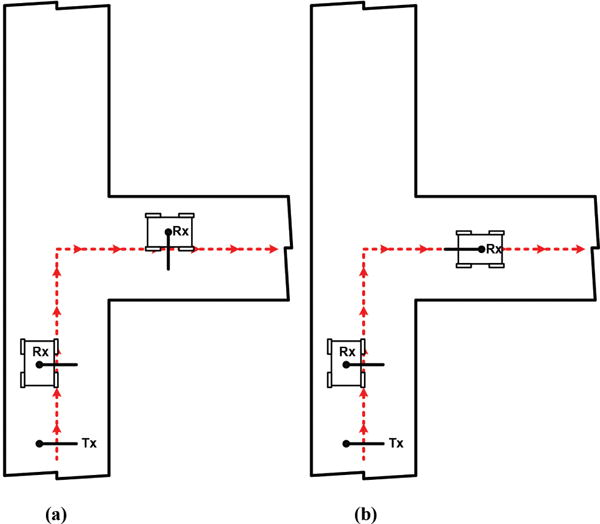
\includegraphics[width=0.35\textwidth]{immagini/corner_em.jpg}
    \caption{Mappa Tunnel U.S. National Institure for Occupational Safety and Health's\citep{jacksha2016}.}
    \label{fig:esempio}
\end{figure}
Mentre
Akyildiz et al. \citep{akyildiz2006} descrivono le difficoltà intrinseche alla
propagazione sotterranea a causa di permittività e conducibilità elevate del terreno.

Più in generale, le tecnologie wireless pensate per ambienti sotterranei devono
fare i conti con una ridotta penetrazione delle frequenze tradizionalmente usate
per IoT. Per questo, l'uso di frequenze estremamente basse (VLF, tra 3–30 kHz)
è stato studiato in scenari di emergenza e applicazioni militari, ma presenta
limiti di banda e di miniaturizzazione delle antenne \citep{salam2023survey}.
\subsection{Onde acustiche}
Un'alternativa promettente alla comunicazione elettromagnetica in ambienti sotterranei è l'impiego di \emph{onde acustiche} (meccaniche), che si propagano attraverso solidi e fluidi (aria, acqua, fanghi di perforazione). A differenza delle onde EM, la propagazione acustica è spesso meno sensibile alla conducibilità elettrica del mezzo e può seguire percorsi guidati (ad es.\ lungo tubazioni o gallerie), con migliore resilienza a curve e biforcazioni \citep{fishta2023inpipe,heifetz2017pipes,farai2023mdpe}.

\paragraph{Modello di canale (cenni).}
Nei \textbf{solidi} (roccia, calcestruzzo, metalli, polimeri), la propagazione è dominata da onde elastiche (longitudinali e di taglio) e, in geometrie guidate 
(tubi, piastre, travi), da \emph{guided waves} (p.\,es.\ onde di Lamb o creep waves) con attenuazione che cresce fortemente con la frequenza e 
con il disaccoppiamento modale \citep{heifetz2020shear}.\\ Nei \textbf{fluidi} in condotti (acqua/aria), il canale è tipicamente 
a bassa frequenza (centinaia di Hz–pochi kHz), con riflessioni multiple e dispersione; in vasche o condotti lunghi si osservano fenomeni di riverbero 
e frequenze di taglio dei modi guida \citep{fishta2023inpipe}. \\Nel \textbf{suolo sfuso} (soil), la trasmissione è di tipo acustico/seismico: 
l’attenuazione dipende da tessitura, umidità e compattazione, ed è marcata oltre poche decine di metri; lo \emph{sweet spot} operativo è in genere 
sotto i 2–5~kHz per massimizzare SNR a parità di potenza \citep{yang2020soil,raza2020wuc}.

\paragraph{Hardware e trasduttori.}
Sono impiegati trasduttori piezoelettrici o magnetostrittivi accoppiati meccanicamente al mezzo (collari su tubi, inserti su rocce/pareti, piastre di accoppiamento).\\
 Nei tubi metallici, coppie di attuatori/ricevitori clamp-on permettono comunicazione non invasiva (senza rompere il tubo), sfruttando onde di taglio o di Lamb \citep{heifetz2017pipes,heifetz2020shear}.\\
  Su polimeri (es.\ tubi MDPE), l’accoppiamento è più debole e la banda utile è più bassa, ma resta praticabile \citep{farai2023mdpe}. \\
  Nei fluidi, si usano idrofoni/speaker impermeabilizzati; nel suolo, trasduttori sismici compatti e miniaturizzati sono stati dimostrati in prototipi a bassa potenza \citep{yang2020soil}.

\paragraph{Tecniche di modulazione e codifica.}
Dato il canale fortemente dispersivo e soggetto a multi-percorso, si adottano modulazioni robuste:
FSK/MFSK e BFSK a bassa frequenza per collegamenti affidabili a bassa velocità; OFDM con stime del canale per massimizzare efficienza in condotti lunghi; e codifica con interleaving e rateless/LDPC per gestire \emph{burst errors} \citep{fishta2023inpipe,farai2023mdpe}. In tubazioni e solidi guidati, è utile la \emph{modal selection} (scegliere il modo meno attenuato) e la \emph{sub-carrier spacing} adeguata alle \emph{delay spreads} misurate \citep{heifetz2020shear,farai2023mdpe}.

\paragraph{Prestazioni riportate in letteratura.}
Risultati sperimentali rappresentativi includono:
\begin{itemize}
    \item \textbf{Suolo (through-soil).} Collegamenti fino a $\sim$50\,m con $\sim$20\,bps utilizzando portanti a bassa frequenza e trasduttori compatti; dimostrazione di comunicazione digitale robusta in campi prova agricoli \citep{yang2020soil}. Survey recenti confermano che, per distanze $>$10–20\,m, le velocità realistiche sono dell’ordine di 1–100\,bps, con forte dipendenza dal contenuto d’acqua \citep{raza2020wuc,acm2023wusn}.
    \item \textbf{Tubi metallici (acciaio).} Trasmissione di dati via onde elastiche lungo tubazioni esistenti in impianti industriali; dimostrate immagini e pacchetti a centinaia di bps–pochi kbps su decine–centinaia di metri a bassa potenza, sfruttando onde di taglio e di Lamb \citep{heifetz2017pipes,heifetz2020shear}.
    \item \textbf{Tubi in polimero (MDPE).} Misure analitiche/numeriche e in campo mostrano che con segnali a bassa frequenza si ottengono distanze utili per telemetria (decine–centinaia di metri) con bitrate modesto (decine–centinaia di bps) \citep{farai2023mdpe,farai2021phd}.
    \item \textbf{Condotti idrici reali.} Revisione dei test in reti idriche urbane indica fattibilità di reti acustiche in-pipe per monitoraggio/IoT, con vincoli di potenza, sincronizzazione e instradamento; lo stato dell’arte è pre-commerciale ma in rapida evoluzione \citep{fishta2023inpipe}.
    \item \textbf{Fluido non convenzionale: fango di perforazione.} Sistemi \emph{while drilling} usano la colonna di fluido come canale acustico per telemetria a bassa velocità (bps–decine di bps) su centinaia di metri, con elevata robustezza \citep{zheng2023mud}.
\end{itemize}

\section{Applicazione della letteratura alla tesi}
La tesi si occuperà quindi della creazione di un protocollo di comunicazione acustica per sistemi distribuiti in ambienti sotteranei, 
basandosi sui risultati e le tecniche di cui sopra, è possibile quindi dedurre alcuni requisiti chiave:
Il protocollo opera nella banda 1–9 kHz. Questa scelta è coerente con la letteratura, che evidenzia come nei condotti fluidi l’impiego di frequenze basse consenta di estendere la portata e ridurre l’attenuazione, fenomeno particolarmente critico per le frequenze più elevate \citep{fishta2023inpipe}
